\section{Validação de projeto}
\label{sec:validacao}

Ao longo do texto, definiu-se os requisitos e como os atingi-los, porém ainda é
preciso estabelecer como ocorrerá a prova do cumprimento do que foi acordado.
Para isso, nessa seção serão propostos alguns testes que são capazes de validar
o cumprimento dos requisitos. Essa etapa de validação poderia ser executada
somente após o desenvolvimento do protótipo, contudo, quaisquer modificações
de projeto com o protótipo já finalizado acrescentaria em um grande custo de
financeiro e em atraso de projeto. Dessa forma, optou-se pela validação do
protótipo via simulação, o que permite testar o veículo em ambiente subaquático
simulado, sem risco de dano ao veículo e evitando grandes retrabalhos por
modificações no projeto. Nessa seção, será discutido como a simulação deve ser
realizada para validação dos requisitos de projeto, assim como a configuração do
ambiente virtual submarino.

\subsection{Módulos de simulação}
\label{sec:simu-modules}

A simulação fidedigna de um veículo submarino deve contar com a simulação dos
atuadores, sensores e da física de um corpo rígido debaixo d'água. Com o objetivo de obter uma simulação que incluísse todos esses tópicos, algumas soluções de \textit{software} disponíveis serão adotas e algumas desenvolvidas, a especificação de cada uma e justificativa de escolha é o objetivo desta seção.

\subsubsection*{Sensores, atuadores e física}

As funções de simular o comportamento de um robô no meio com seus sensores e
atuadores é a tarefa de um simulador de robótica, dessa forma, é necessário se
definir qual deve ser utilizado para a validação deste projeto. A tabela da
Figura \ref{fig:simulators-comparison} mostra as alternativas de simuladores
que possuem funcionalidades essenciais para validação de um robô submarino.
Dentre as cinco alternativas apresentadas na tabela, 3 delas utilizam o simulador Gazebo \cite{gazebo}, que são UWSim ({\it Underwater Simulator}), UUV
({\it Unmanned Underwater Vehicle Simulator}) e USVSim ({\it Unmanned Surface
Vehicle Simulator}). Dentre esses, o USVSim seria o mais completo, pois dispoẽ
de quase todas as funcionalidades apresentadas na Figura \ref{fig:simulators-comparison}.

\begin{table}[h]
    \label{tab:simulators-comparison}
    \caption{Tabela comparativa de simulatores e suas funcionalidades}
    \centering
    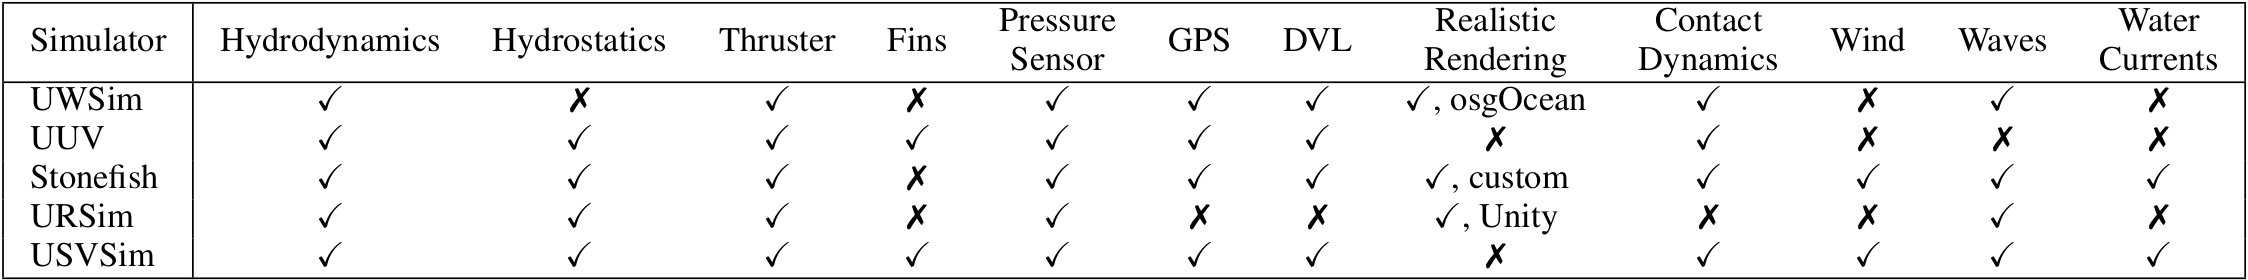
\includegraphics[width=1\textwidth]{images/simulators_comparison.png}\\
    \footnotesize Fonte: \cite{simulators-comparison}
\end{table}

Contudo, o USVSim é desenvolvido a partir do Gazebo, então seria necessário a
instalação de duas ferramentas, sendo que a Open Robotics, empresa desenvolvedora do Gazebo, lançou o novo simulador que substituirá o Gazebo, o
Ignition. Ademais, o Ignition já apresenta as funcionalidades de robótica
submarina incorporadas, dessa forma, optou-se por utilizar somente o \textit{software} Ignition. Nele é possível se carregar um ambiente submarinho 3D assim como o veículo, sendo possível não somente a visualização, mas também obter dados simulados de sensores, controlar motores e simular a interação do robô com o ambiente ao seu redor.

\subsubsection*{Comunicação e sensor de distância acústicos}
Apesar do Ignition possibilitar a simulação dos motores e sensores do veículo, a simulação da comunicação e sensor de distância acústicos é uma funcionalidade que não consta no \textit{software}. Portanto, serão desenvolvidos \textit{plugins} para o \textit{software} que simulam as peculiaridades desse tipo sensores. Os \textit{plugins} devem simular atraso da onda sonora na água, ruído e atenuação.

É extremamente caro e complexo implantar uma estrutura completa de rede subaquática com links de dados para coletar e transmitir informações de uma coluna de água, composta por nós de sensores, gateways na superfície e AUVs \cite{godi2021survey}. Pois, os dispositivos custam caros devidos a baia de proteção, são propensos a falhas por causa da corrosão e incrusto, as baterias limitadas não podem ser recarregadas com energia solar e a manutenção é complicada por estarem submersos \cite{akyildiz2005underwater, shantaram2005challenges}.

Além do mais, é difícil validar os protocolos ou algoritmos usados na rede UWSN por meio de testes, os planos de testes implantados podem não ser adequado para todos os tipos de aplicações, implementação repetida afeta os resultados experimentais e ainda é demorada \cite{das2016simulation}.  

Diante do exposto acerca dos desafios citados, a existência de um ambiente de simulação que replicasse o cenário subaquático real, permitiria ao engenheiro ou pesquisador estudar os comportamentos com base nas características físicas, por meio dos testes de seus modelos em par com a implementação em tempo real.

Para simular a comunicação, no presente trabalho será utilizado a biblioteca de simulação escrita em Python que objetiva testar algoritmos de rede acústica chamada AUVNetSim: A Simulator for Underwater Acoustic Networks produzido pelo \cite{montana2008auvnetsim} em um programa no MIT(do inglês, Massachusetts Institute of Technology) em 2008. O pacote contém uma grande variedade parâmetros e protocolos para redes acústicas subaquáticas que podem ser selecionadas ou modificados para implementar novos protocolos aproveitando a estrutura existente.

Além disso, na simulação de cada nó acústico a comunicação é realizada por troca de mensagens curtas entre as camadas que podem ser configuradas na seguinte ordem: física, MAC, roteamento e aplicação conforme é apresentado na Figura \ref{fig:auvnetsim} logo abaixo.

\begin{figure}
	\centering
	\caption{Estrutura de programação de um nó acústico AUVNetSim}
	\label{fig:auvnetsim}
	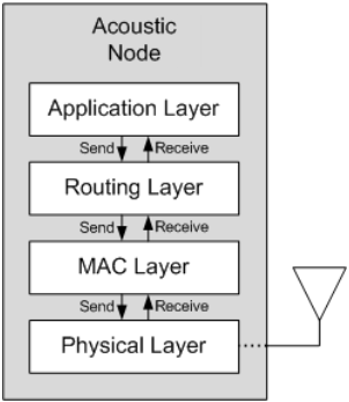
\includegraphics[width=0.3\linewidth]{images/auvnetsim}\\
	\footnotesize Fonte: \cite{montana2008auvnetsim}
\end{figure}

Apesar de existirem outras propostas de ferramentas disponíveis no mercado com mesma característica e até melhores que o AUVNetSim, como Network Simulator (NS-3), SUNSET ou Aqua-Sim que permitem além da emulação, testes em tempo real \cite{godi2021survey} o que aproximaria ainda mais do sistema mais realista . Entretanto, a biblioteca foi selecionada por ser de código aberto e mesmo que ainda não testada a fundo, apresenta-se através do manual de utilização \cite{montana2008auvnetsim} que é de fácil integração e manutenção, os pré-requisitos não exigi recursos computacionais muito pesados para a sua utilização, e a curva de aprendizado é reduzida em comparação a outras opções e o prazo de entrega do projeto.

Assim, à adoção do AUVNetSim tem como objetivo integrá-la com Robot Operating System (ROS), com a finalidade de simular a comunicação entre os dispositivos em uma topologia de rede com a arquitetura tridimensional com AUV conforme proposta apresentada na Figura \ref{fig:redes}. Do mesmo modo, ainda serão estudados, avaliados e testados outros protocolos propostos na literatura com o propósito de se obter uma configuração satisfatória e que se aproxime do mundo real na simulação de como o todo.

\begin{figure}
	\centering
	\caption{Arquitetura de comunicação subaquática}
	\label{fig:redes}
	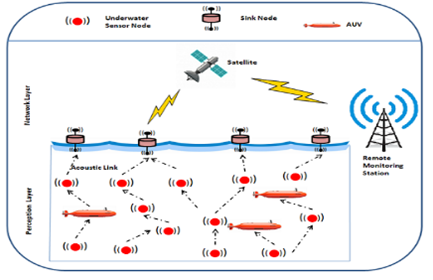
\includegraphics[width=0.7\linewidth]{images/redes}\\
	\footnotesize Fonte: \cite{godi2021survey}
\end{figure}



\subsection{Missões}

As missões são tarefas definidas para validação das funcionalidades do veículo, de forma que ao cumprir cada missão, o projeto fica validade a nível de simulação para o cumprimento dos requisitos de projeto.

\subsubsection*{Submersão e emersão controlada}
Essa missão consiste em submergir e emergir o ROV a uma determinada profundidade,
como pode ser visto na Figura \ref{fig:descent-test}. Esse procedimento será executado tanto com controle manual de velocidade, como também com controle automático, no qual o ROV se desloca ao longo de um caminho previamente estabelecido. Além disso, arucos seriam posicionados ao longo de todo o trajeto, para obter uma medição mais precisa de profundidade.

\begin{figure}[h]
	\label{fig:descent-test}
	\caption{Missão de submersão e emersão}
	\centering
	\includegraphics[width=0.8\textwidth]{images/descent_test.png}
\end{figure}

Dessa forma, os requisitos 2, 6 e 7 seriam validados, visto que para a execução dessa tarefa, o ROV deve ser capaz de ir para uma posição previamente conhecida, localizar os arucos e submergir e emergir de forma controlada.

\subsubsection*{Teste de velocidade e trajetória circular}

O requisito 3 determina a velocidade máxima que o veículo deve atingir, então é necessário que haja algum teste em que os motores do veículo fiquem no seu máximo para verificar se a velocidade determinada consegue ser atingida. O ROV foi projetado para ter mais velocidade em \textit{surge}, de forma a se deslocar mais rápido ao se mover para frente. Dessa forma, o teste de velocidade consiste em colocar a referência de velocidade no seu valor máximo e medir a velocidade de deslocamento do ROV nesse trecho, porém essa medição é pouco precisa com a configuração de sensores atuais.

Portanto, para medir a velocidade, serão posicionados arucos de diferentes tamanhos e o sistema de SBL. A configuração do ambiente de teste pode ser observada na Figura \ref{fig:speed-test}. Os arucos tem tamanho variado pois quanto maior o aruco, mais longe deve-se estar para medir sua pose com precisão, então arucos de diferentes tamanhos servirão para ter uma boa medição em um intervalo maior de distância do veículo para o aruco.

\begin{figure}[h]
	\label{fig:speed-test}
	\caption{Missão de velocidade máxima e seguimento de trajetória}
	\centering
	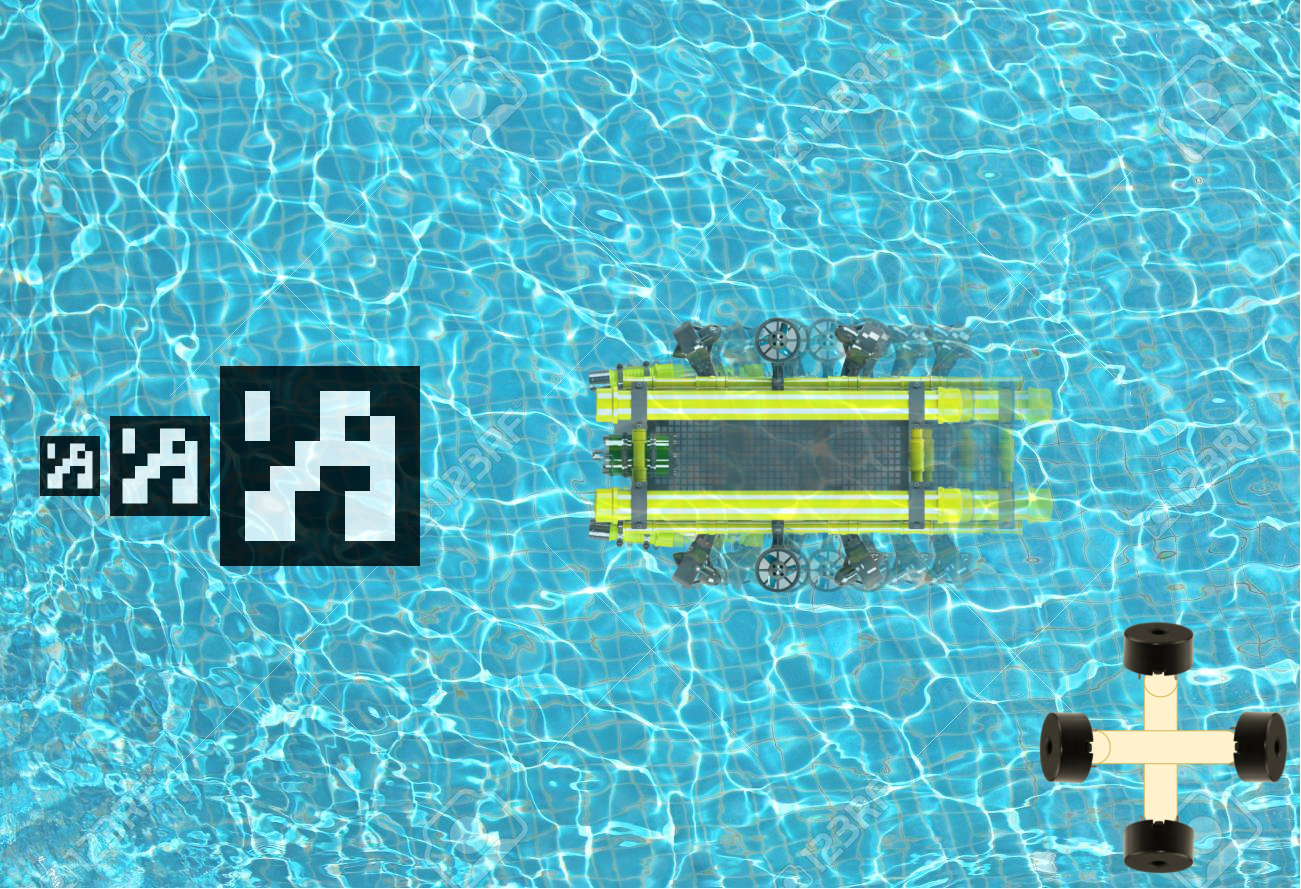
\includegraphics[width=0.8\textwidth]{images/speed_test.png}
\end{figure}

Outra missão que será executada nessa mesma configuração é a execução de uma trajetória circular, para validação dos requisitos 4, 6 e 7. Ao se executar a trajetória circular, mantendo a profundidade e mantendo os arucos no campo de visão da câmera, pode-se usar o armazenamento da trajetória para validar se o requisito de seguir uma trajetória realmente foi cumprido.

\subsubsection*{Mapeamento de rampa}

A validação do requisito 5, que se refere ao mapeamento do leito marinho, pode ser
validado ao se utilizar um terreno conhecido. Então, propõe-se aqui a execução do simples mapeamento de uma rampa, caso a inclinação da rampa seja semelhante ao do mapeamento, pode-se afirmar que o sistema funciona. O mapeamento não será muito detalhado, visto que irá se adquirir somente informação de 4 pontos, medidos com sensores de distância ultrassom abaixo do ROV. Portanto um cenário simples como uma rampa é adequado para validação. Além disso, também se necessita do aruco para posicionamento do ROV, como na Figura \ref{fig:mapping-test}.

\begin{figure}[h]
	\label{fig:mapping-test}
	\caption{Missão de mapeamento}
	\centering
	\includegraphics[width=0.8\textwidth]{images/mapping_test.png}
\end{figure}

\subsubsection*{Resgate da Moeda}
As missões apresentadas até agora cobriram a validação de todos os requisitos de sistemas que não envolvem resistência e confiabilidade, a validação que está faltando quanto a funcionalidade é a 8. Esse requisito determina que o ROV deve ser capaz de atender um pedido de socorro. Para a validação desse requisito, o BROV deve localizar a caixa de resgate, representada pelo aruco mais à esquerda da Figura \ref{fig:object-retrieving-test}. Além disso, deve esperar o led presente na caixa ascender, a partir daí, o ROV deve se aproximar e capturar a moeda com seu imã e retornar a superfície. Esse teste não só valida o requisito 8, mas como todos os citados anteriormente, a ideia é testar o sistema atendendo todos os requisitos funcionais do ROV ao mesmo tempo. Para esse teste, tanto a localização por aruco como a por SBL .

\begin{figure}[h]
	\label{fig:object-retrieving-test}
	\caption{Tabela comparativa de simulators e suas funcionalidades}
	\centering
	\includegraphics[width=0.8\textwidth]{images/object_retrieving_test.png}
\end{figure}


